% Shared TikZ scaffold for OpenResearch figures.
%
% Compile on its own (`\documentclass{standalone}` writes a tightly cropped PDF
% next to the source), or copy the \definecolor and \tikzset blocks into a
% paper's preamble and \input the tikzpicture directly.
%
% The colors are the same Okabe-Ito values as orx_figstyle.PALETTE, so a
% diagram and a plot in the same paper agree on what "ours" is colored.

\documentclass[border=2pt]{standalone}
\usepackage{tikz}
\usepackage{amsmath}
\usetikzlibrary{arrows.meta, positioning, fit, backgrounds, calc, shapes.geometric}

% Diagram text is sans, matching the matplotlib figures next to it — figure
% text is its own typographic register and should be consistent across the
% paper's figures, not with the body text. The face is set per style below,
% never with \familydefault, which would follow this preamble into a paper and
% turn its body text sans too. For a serif diagram to match plots built with
% use_style(family="serif"), drop the \sffamily from the three font= styles.

\definecolor{orxblue}{HTML}{0072B2}
\definecolor{orxorange}{HTML}{E69F00}
\definecolor{orxgreen}{HTML}{009E73}
\definecolor{orxred}{HTML}{D55E00}
\definecolor{orxpurple}{HTML}{CC79A7}

\tikzset{
  % Every picture starts from this: one arrow tip, one line weight, one font.
  orx/.style={
    font=\sffamily\footnotesize,
    >={Stealth[round, length=4pt, width=3pt]},
    line width=0.5pt,
    node distance=6mm and 14mm,  % wide enough for a shape label on the edge
  },
  % A computation: something with parameters or a transform.
  block/.style={
    draw=black!55, fill=white, rounded corners=1pt,
    minimum height=6.5mm, minimum width=15mm, inner sep=3pt, align=center,
  },
  % The contribution. Exactly one kind of thing in a figure should be accented.
  ours/.style={block, draw=orxblue, fill=orxblue!7, line width=0.7pt},
  % Context that must be present but is not the point.
  muted/.style={block, draw=black!30, fill=black!3, text=black!65},
  % A tensor, dataset, or artifact rather than an operation.
  data/.style={
    draw=black!45, fill=black!4, trapezium, trapezium left angle=72,
    trapezium right angle=108, trapezium stretches body,
    minimum height=6mm, inner sep=3pt, align=center,
  },
  flow/.style={->, draw=black!65},
  % A gradient, stop-gradient, or otherwise non-forward path.
  backflow/.style={->, draw=orxorange, dashed},
  % Shapes, losses, and other annotations that ride on an edge.
  edgelbl/.style={font=\sffamily\scriptsize, text=black!60, inner sep=1.5pt, fill=white},
  % A named stage grouping several blocks.
  stage/.style={draw=black!25, dashed, rounded corners=2pt, inner sep=4pt},
  stagelbl/.style={font=\sffamily\scriptsize\itshape, text=black!55},
}

% SCA method diagram. Compile: tectonic --outdir .. method.tex  (writes ../method.pdf)
\begin{document}
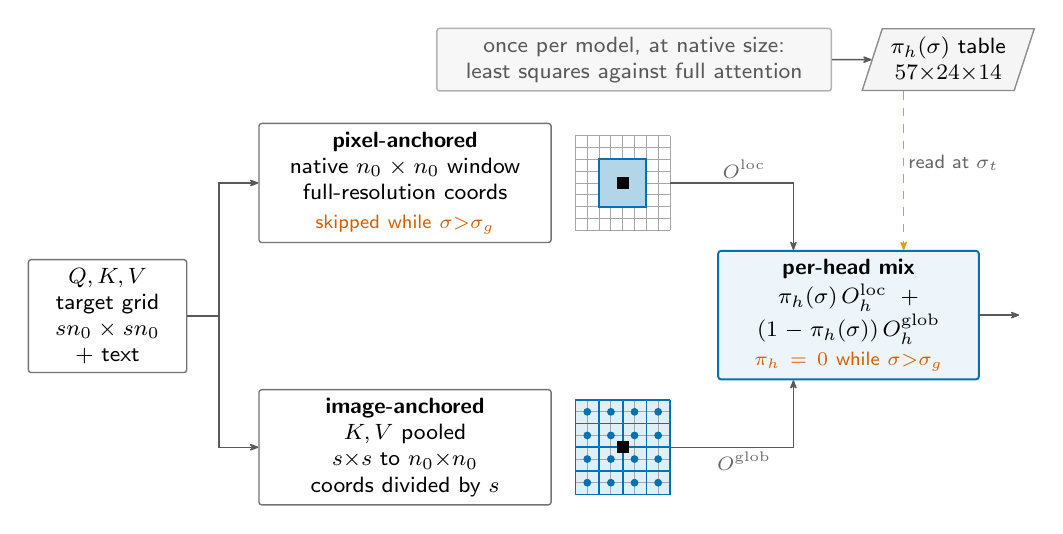
\begin{tikzpicture}[orx, node distance=5mm and 8mm]

  % one attention layer at the target grid
  \node[block, text width=18mm] (qkv) {$Q,K,V$\\target grid\\$sn_0\times sn_0$\\+ text};

  % pixel-anchored branch (skipped while the noise gate is closed)
  \node[block, above right=2mm and 9mm of qkv, text width=35mm] (loc)
    {\textbf{pixel-anchored}\\native $n_0\times n_0$ window\\full-resolution coords\\[1pt]{\scriptsize\color{orxred}skipped while $\sigma{>}\sigma_g$}};
  % image-anchored branch
  \node[block, below right=2mm and 9mm of qkv, text width=35mm] (glob)
    {\textbf{image-anchored}\\$K,V$ pooled $s{\times}s$ to $n_0{\times}n_0$\\coords divided by $s$};
  \draw[flow] (qkv.east) -- ++(4mm,0) |- (loc.west);
  \draw[flow] (qkv.east) -- ++(4mm,0) |- (glob.west);

  % receptive-field sketches: black = query, blue = keys it sees
  \begin{scope}[shift={($(loc.east)+(3mm,-6mm)$)}, x=1.5mm, y=1.5mm]
    \draw[black!35, line width=0.3pt] (0,0) grid[step=1] (8,8);
    \fill[orxblue!30] (2,2) rectangle (6,6);
    \draw[orxblue, line width=0.7pt] (2,2) rectangle (6,6);
    \fill[black] (3.5,3.5) rectangle (4.5,4.5);
    \coordinate (locsk) at (8,4);
  \end{scope}
  \begin{scope}[shift={($(glob.east)+(3mm,-6mm)$)}, x=1.5mm, y=1.5mm]
    \fill[orxblue!12] (0,0) rectangle (8,8);
    \draw[black!35, line width=0.3pt] (0,0) grid[step=1] (8,8);
    \draw[orxblue, line width=0.6pt] (0,0) grid[step=2] (8,8);
    \foreach \i in {1,3,5,7} \foreach \j in {1,3,5,7} \fill[orxblue] (\i,\j) circle (0.33);
    \fill[black] (3.5,3.5) rectangle (4.5,4.5);
    \coordinate (globsk) at (8,4);
  \end{scope}

  % per-head mixing
  \coordinate (mixin) at ($(locsk)!0.5!(globsk)+(6mm,0)$);
  \node[ours, anchor=west, text width=31mm] (mix) at (mixin)
    {\textbf{per-head mix}\\[1pt]$\pi_h(\sigma)\,O^{\mathrm{loc}}_h\;+$\\$(1-\pi_h(\sigma))\,O^{\mathrm{glob}}_h$\\[1pt]{\scriptsize\color{orxred}$\pi_h=0$ while $\sigma{>}\sigma_g$}};
  \draw[flow] (locsk) -| node[edgelbl, pos=0.3, above] {$O^{\mathrm{loc}}$} ($(mix.north)+(-7mm,0)$);
  \draw[flow] (globsk) -| node[edgelbl, pos=0.3, below] {$O^{\mathrm{glob}}$} ($(mix.south)+(-7mm,0)$);
  \draw[flow] (mix.east) -- ++(5mm,0);

  % offline calibration, once per model
  \coordinate (tabx) at ($(mix.north)+(7mm,0)$);
  \coordinate (tabpos) at ($(mix.north east |- loc.north)+(0,4mm)$);
  \node[data, anchor=south east] (table) at (tabpos) {$\pi_h(\sigma)$ table\\$57{\times}24{\times}14$};
  \draw[backflow] (table.south -| tabx) -- node[edgelbl, right, pos=0.45] {read at $\sigma_t$} (tabx |- mix.north);
  \node[muted, left=5mm of table, text width=48mm] (calib)
    {once per model, at native size:\\least squares against full attention};
  \draw[flow] (calib) -- (table);

\end{tikzpicture}
\end{document}
